\subsection{Use Case}
\label{sec:usecase}

The use cases from figure \ref{tab:actoreventtable} are described below.  

\paragraph{\ucsproblem[c]} The use case \ucsproblem[] is only used by the actor \aclient. Except for cases when \astaff{} or \sadmin{}  acts as \aclient{}. A use case diagram is shown in figure \ref{fig:submit_problem_use_case}. 
\begin{itemize}
\item \sadb{Use Case:} \ucsproblem[c] is initialized when a \aclient{} has a problem and wishes to submit that problem to the system in order to get help from the \astaff{}. 
First he has to select a category and choose one or more tags, he can select tags from more then one category. 
When the \aclient{} is done selecting tags the system compares the selected tags with other problems. 
If similar problems is found the \aclient{} is presented with these.
If one of these matches his particular problem, he can subscribe to the problem if it is \open[] or read the solution(s) if the problem is \closed{}, thus hoping that this will lead to solving the \aclient s problem.
If no similar problem was found the \aclient{} creates a problem with a title, description and the previously selected tags. 
Hereafter the problem gets assigned to a \astaff{}. 

\item \sadb{Objects:} \cl{Problem, tag, category, \aclient[], \astaff[]}.

\item \sadb{Functions:} Get problem tags, Search for problems, Create problem, Subscribe / unsubscribe to problem, and Get Est. Time Consumption of Problem. 
\end{itemize}

\begin{figure}[htbp]
\begin{center}
 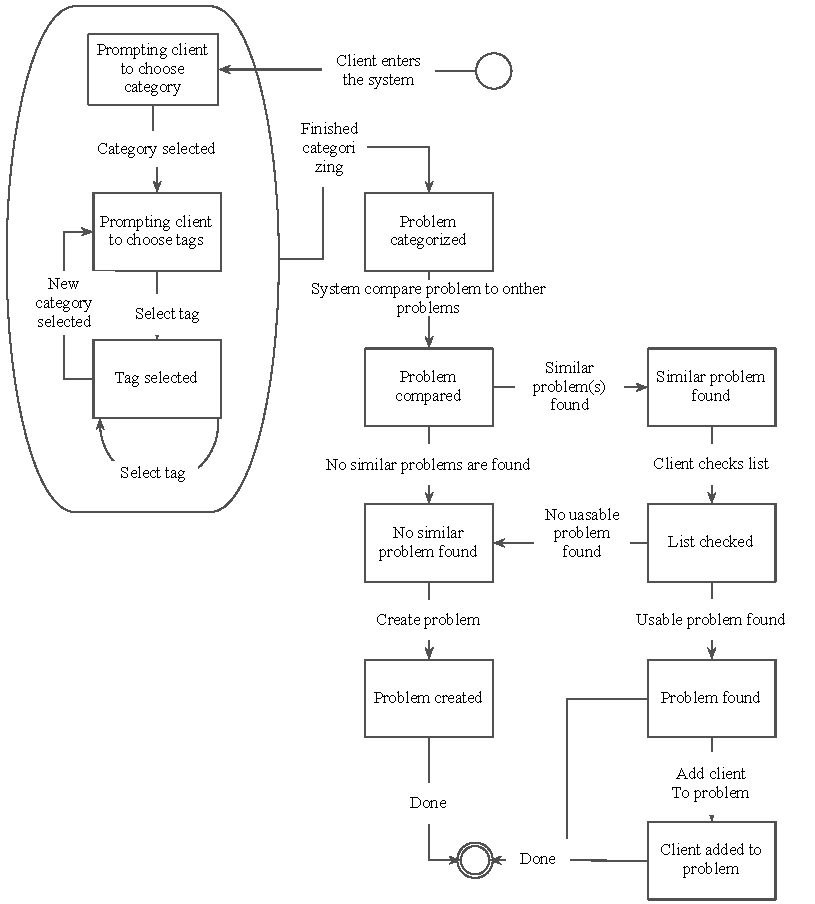
\includegraphics[scale=0.8]{input/application_domain_analysis/submit_problem_use_case}
\morscaption{A state chart diagram of the use case \ucsproblem{}.}
\label{fig:submit_problem_use_case}
\end{center}
\end{figure}

\paragraph{My problems} The use case my problems is used by  \aclient s, \astaff s, and \admin s. It show a list all problems submitted by the user. From there details can be viewed for each problem. 

%\paragraph{\bloadwork[c]} \bloadwork[c] is the operation of the \wmon{}. It checks and compares all staff members workload and redistribute problems in order to equally balance the workload in each department. 

\paragraph{\gstat[c]} The use case \gstat[] is accessible by the \admin[]. It shows statistics about how much time each \astaff[] use to solve problems.

\paragraph{\ucsolproblem[c]} The use case \ucsolproblem{} is the \astaff{}s primary usage of the system. When the \astaff[] get his \todolist[] he can select a problem and solve the problem. A statechart diagram is shown in figure \ref{fig:solve_problem_use_case}.

\begin{itemize}
\item \sadb{Use Case:} The use case is initialized when the \astaff[] wants to check his \todolist[]. The \astaff[] is then presented with a list of unsolved problems assigned to him. The \astaff[] can then click on one of the problems to read the problem, see status of it, add comments to it, search the database for similar problem, reassign it, or write a new solution. 

\item \sadb{Objects:} Problem, solution, comment, \client[], and \staff[].
fixme{staff must at least have the same objects as client}

\item \sadb{Functions:}Get problem tags, Search for problems, Create problem, Subscribe / unsubscribe to problem, Get est. time consumption of problem, Manage tag times, Get expected time of completion of problem, Get tag average time consumption, Get sorted worklist and Approve deadline. 


 Add comment, reassign, change status, search database, create solution, attach solution and get staff \todolist{}.
\end{itemize}

\begin{figure}[htbp]
\begin{center}
 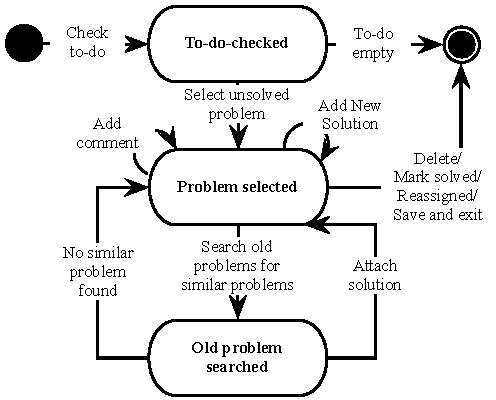
\includegraphics[scale=0.8]{input/application_domain_analysis/solve_problem_use_case}
\morscaption{A state chart diagram of the use case \ucsolproblem{}.}
\label{fig:solve_problem_use_case}
\end{center}
\end{figure}

\paragraph{\tucadmin[c]} The use case \tucadmin[] is used by the \sadmin[] to administrate persons, tags, categories, departments and view statistics about the specific \astaff members. A statechart diagram is depicted on figure \ref{fig:use_case_diagram}.

\begin{itemize}
\item\sadb{Use Case:} The use case starts as the \sadmin{} enters the site. The \admin[] can manage people by change role, department, email and delete the person from the system. The \admin[] is also able to create new  departments and add categories thereto. To each category new tags can be added. Tags have a priority which can be changed at anytime. Tags cannot be removed when they have been used, but they can be hidden so they cannot be used to categories new problems.  

\item\sadb{Objects:} \cl{ \staff[c], \client[c], category, tag, department}. 
\fixme{admin must at least have the same objects as client}

\item\sadb{Functions:} Get problem tags, Search for problems, Create problem, Subscribe / unsubscribe to problem, Get est. time consumption of problem, Manage tag times, Get expected time of completion of problem, Get tag average time consumption, Get sorted worklist, Approve deadline, Create department, Create category, Create tag, Hide / show category, Hide / show tag, Delete person, Reset person password, Balance workload, Get statistics, and Distribute problem. 
\end{itemize}


\begin{figure}[htbp]
\begin{center}
 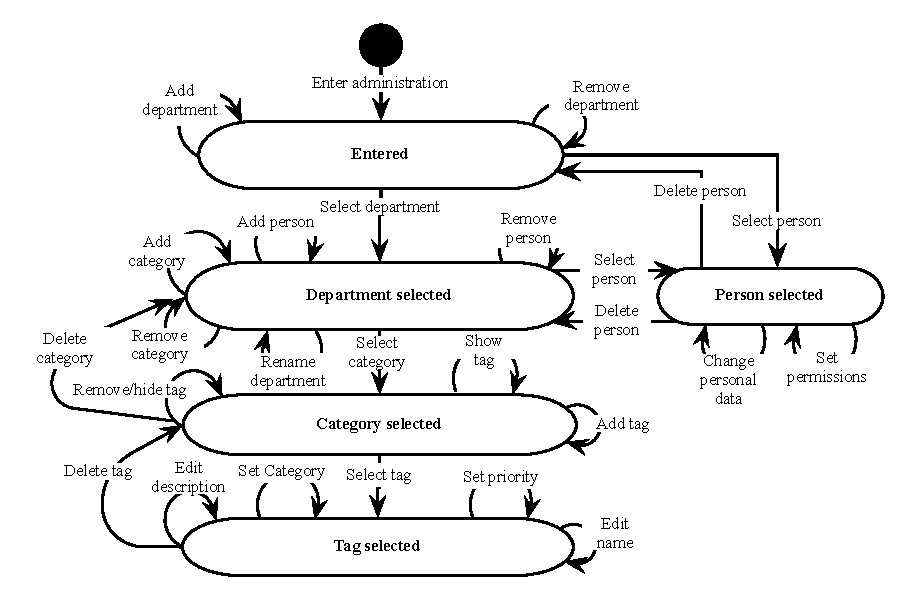
\includegraphics[scale=0.8]{input/application_domain_analysis/admin_use_case}
\morscaption{A statechart diagram for the use case \tucadmin{}.}
\label{fig:use_case_diagram}
\end{center}
\end{figure}